\chapter{Espacios euclídeos}

\begin{definicion}[Espacios euclídeos]
    Diremos que un espacio afín $E$ es euclídeo si $\vec{E}$ está dotado de la estructura euclídea. Es decir, $(\vec{E},~\langle,\rangle)$.
\end{definicion}


\begin{definicion}[Distancia]
    Sea $E$ un espacio euclídeo. Definimos la aplicación distancia dada por:
    \Func{d}{E\times E}{\bb{R}}{(p,q)}{d(p,q)=\|\vec{pq}\|=\sqrt{\langle\vec{pq},\vec{pq}\rangle}}
\end{definicion}

Tenemos que la aplicación anterior es, efectivamente, una distancia, ya que:
\begin{enumerate}
    \item $d(p,q)\geq 0~~\forall p,q\in E$. Además, $d(p,q)=0\Longleftrightarrow p=q$.
    \item $d(p,q)=d(q,p)~~\forall p,q\in E$.
    \item $d(p,q)\leq d(p,r) + d(r,q)~~\forall p,q,r\in E$.
\end{enumerate}

\begin{definicion}
    Sean $S,T$ dos subespacios afines de $E$ espacio euclídeo. Entonces, definimos que $S$ y $T$, notado por $S\perp T$, si y solo si:
    \begin{equation*}
        S\perp T \Longleftrightarrow \vec{S}\perp \vec{T}
    \end{equation*}
\end{definicion}

\begin{teo}
    Sea $E$ un espacio euclídeo, y sea $S$ un subespacio afín de $E$. Entonces, $\forall q\in E$, $\exists_1 T$ subespacio afín de $E$ verificando:
    \begin{enumerate}
        \item $q\in T$,
        \item $T\perp S$,
        \item $\dim T + \dim S = n=\dim E$.
    \end{enumerate}
\end{teo}
\begin{proof}
    Como $\dim \vec{T} + \dim \vec{S} = \dim \vec{E}$, y se tiene que $\vec{T}\perp \vec{S}$, se tiene que $\vec{T}=\vec{S}^\perp$.
    
    Por tanto, definimos el subespacio $T$ buscado como:
    $$T=q+\vec{S}^\perp$$

    Tenemos por tanto demostrada la existencia. La unicidad se tiene de forma directa, ya que $\vec{S}^\perp$ es único. Por tanto, para cada $q\in E$, tenemos que $T$ es único.
\end{proof}

Este teorema da lugar a la siguiente definición:
\begin{definicion}
    Sea $E$ un espacio euclídeo, y sea $S$ un subespacio afín de $E$. Entonces, dado $q\in E$, definimos el subespacio ortogonal a $S$ que pasa por $q$, notado por $S^\perp_q$, como:
    $$S^\perp_q = q+\vec{S}^\perp$$
\end{definicion}



\begin{definicion}
    Sea $E$ un espacio euclídeo. Un sistema de referencia $\cc{R}=\{p_o,\cc{B}\}$ de $E$ diremos que es \ul{euclídeo} si $\cc{B}$ es una base ortonormal.
\end{definicion}

Recordemos el Teorema de Pitágoras, demostrado en Geometría II.
\begin{teo}[de Pitágoras]
    Sea $E$ un espacio euclídeo. Dados $a,b,c\in E$, se tiene que:
    \begin{equation*}
        \|\vec{ac}\|^2 + \|\vec{ab}\|^2 = \|\vec{cb}\|^2 \Longleftrightarrow \vec{ac}\perp \vec{ab}
    \end{equation*}
    \begin{figure}[H]
        \centering
        \begin{tikzpicture}[scale=0.6]
            % Define los vértices del triángulo
            \coordinate (A) at (0,0);
            \coordinate (B) at (7,0);
            \coordinate (C) at (0,3);
        
            % Dibuja el triángulo
            \draw (A) -- (B) -- (C) -- cycle;
        
            % Etiqueta los vértices
            \node[below] at (A) {$a$};
            \node[below] at (B) {$b$};
            \node[above] at (C) {$c$};

            \tkzMarkRightAngle[size=0.3](B,A,C)
        \end{tikzpicture}
    \end{figure}
\end{teo}


\begin{definicion}[Mediatriz]
    Sea $E$ un espacio euclídeo. Dado $a,b\in E$, definimos la mediatriz del segmento $\ol{ab}$ como el único subespacio afín perpendicular a la recta que une ambos puntos que pasa por el punto medio. Es decir,
    $$L=r^\perp_M = M + \vec{r}^\perp$$
    donde $r$ es la recta que une $a,b$, es decir, $r=a+\cc{L}\{\vec{ab}\}$; y $M$ es el punto medio de $a$ y $b$, es decir, $M=a+\frac{1}{2}\vec{ab}$.
    \begin{figure}[H]
        \centering
        \begin{tikzpicture}
            \coordinate (A) at (0,0);
            \coordinate (B) at (4,0);
            \coordinate (P) at (2,2);
            
            \draw[dashed] (A) -- (B); % Dibuja el segmento AB
            
            % Mediatriz
            \path (A) -- (B) coordinate[midway] (M); % Punto medio
            \draw[-stealth] (M) -- ($(M)!1.5cm!90:(B)$); % Dibuja la mediatriz
            \draw[-stealth] (M) -- ($(M)!-1.5cm!90:(B)$); % Extiende la mediatriz hacia abajo

            \tkzMarkRightAngle[size=0.3](B,M,P)
        
            % Marcar los puntos con círculos rellenos
            \filldraw (A) circle (2pt) node[anchor=east] {$a$};
            \filldraw (B) circle (2pt) node[anchor=west] {$b$};
            \filldraw (M) circle (2pt) node[anchor=north west] {$M$};
        \end{tikzpicture}
    \end{figure}
\end{definicion}


\begin{prop} Sea $E$ un espacio euclídeo. Dado $a,b\in E$, y dado $p\in E$, se caracteriza la mediatriz de $a,b\in E$ como:
    \begin{equation*}
        p\in r^\perp_M \Longleftrightarrow d(a,p)=d(b,p)
    \end{equation*}
    \begin{figure}[H]
        \centering
        \begin{tikzpicture}
            \coordinate (A) at (0,0);
            \coordinate (B) at (4,0);
            \coordinate (P) at (2,1);
            
            \draw[dashed] (A) -- (B); % Dibuja el segmento AB

            \draw[dashed] (P) -- (A); % Dibuja el segmento AP
            \draw[dashed] (P) -- (B); % Dibuja el segmento BP
            
            % Mediatriz
            \path (A) -- (B) coordinate[midway] (M); % Punto medio
            \draw[-stealth] (M) -- ($(M)!1.5cm!90:(B)$); % Dibuja la mediatriz
            \draw[-stealth] (M) -- ($(M)!-0.5cm!90:(B)$); % Extiende la mediatriz hacia abajo

            \tkzMarkRightAngle[size=0.3](B,M,P)
        
            % Marcar los puntos con círculos rellenos
            \filldraw (A) circle (2pt) node[anchor=east] {$a$};
            \filldraw (B) circle (2pt) node[anchor=west] {$b$};
            \filldraw (M) circle (2pt) node[anchor=north west] {$M$};

            \filldraw (P) circle (2pt) node[anchor=west] {$p$};
        \end{tikzpicture}
    \end{figure}
\end{prop}
\begin{proof}\
    \begin{description}
        \item[$\Longrightarrow)$] Veamos en primer lugar que $\|\vec{Ma}\|=\|\vec{Mb}\|$:
        \begin{gather*}
            \vec{Ma} = a-M=a-a-\frac{1}{2}\vec{ab} = -\frac{1}{2}\vec{ab} \Longrightarrow ||\vec{Ma}|| = \frac{1}{2}\|\vec{ab}\|\\
            \vec{Mb} = b-M=b-a-\frac{1}{2}\vec{ab} = \vec{ab}-\frac{1}{2}\vec{ab} = \frac{1}{2}\vec{ab} \Longrightarrow ||\vec{Mb}|| = \frac{1}{2}\|\vec{ab}\|
        \end{gather*}
        
        
        Veamos ahora que $\vec{pM}\perp \vec{Ma}$. Para ello, vemos que $\vec{Ma}\in \vec{r}$:
        \begin{equation*}
            \vec{Ma}=a-M=a-a-\frac{1}{2}\vec{ab}=-\frac{1}{2}\vec{ab}\in \cc{L}\{\vec{ab}\}
        \end{equation*}
        Análogamente, tenemos que $\vec{Mb}\in \vec{r}$. Además, tenemos que $p,M\in r_M^\perp$, por lo que $\vec{Mp}\in \vec{r}^\perp$. Por tanto, por definición de subespacio ortogonal, tenemos que $\vec{Mp}\perp \vec{Ma},\vec{Mb}$.

        Por tanto, por el Teorema de Pitágoras, tenemos que:
        \begin{equation*}
            \|\vec{pa}\|^2 = \|\vec{Mp}\|^2 + \|\vec{Ma}\|^2 \AstIg \|\vec{Mp}\|^2 + \|\vec{Mb}\|^2 = \|\vec{pb}\|^2
        \end{equation*}
        donde en $(\ast)$ he aplicado que $\|\vec{Ma}\|=\|\vec{Mb}\|$. Por tanto, tenemos que $\|\vec{pa}\|=\|\vec{pb}\|$, por lo que:
        \begin{equation*}
            d(a,p)=\|a-p\| = \|\vec{pa}\|=\|\vec{pb}\| = \|b-p\| = d(b,p)
        \end{equation*}
        
        \item[$\Longleftarrow)$] Supongamos que $p\notin r_M^\perp$, y lleguemos a una contradicción.
        
        Como $p\notin r_M^\perp$, tenemos que $\vec{Mp}\notin \vec{r}^\perp$. Por tanto, $\exists v\in \cc{L}\{\vec{ab}\}$ tal que $\langle v,\vec{Mp}\rangle\neq 0$. Como $v\in \cc{L}\{\vec{ab}\}$, tenemos que $v=k\cdot \frac{1}{2}\vec{ab}$ para cierto $k\in \bb{R}^\ast$. Por tanto,
        \begin{equation*}
            0\neq \langle v,\vec{Mp}\rangle = \left\langle k\cdot \frac{1}{2}\vec{ab},\vec{Mp}\right\rangle
            = k \left\langle \frac{1}{2}\vec{ab},\vec{Mp}\right\rangle
            = k \left\langle \vec{Mb},\vec{Mp}\right\rangle
            = -k \left\langle \vec{Ma},\vec{Mp}\right\rangle
        \end{equation*}

        Por tanto, tenemos que $\vec{Mp}\not \perp \vec{Ma},\vec{Mb}$. Por el Teorema de Pitágoras, tenemos que:
        \begin{equation*}
            \|\vec{pa}\|^2 \neq \|\vec{Mp}\|^2 + \|\vec{Ma}\|^2 \AstIg \|\vec{Mp}\|^2 + \|\vec{Mb}\|^2 \neq \|\vec{pb}\|^2
        \end{equation*}
        donde en $(\ast)$ he aplicado que $\|\vec{Ma}\|=\|\vec{Mb}\|$. Por tanto, tenemos que $\|\vec{pa}\|\neq\|\vec{pb}\|$, por lo que:
        \begin{equation*}
            d(a,p)=\|a-p\| = \|\vec{pa}\|\neq \|\vec{pb}\| = \|b-p\| = d(b,p)
        \end{equation*}
        llegando entonces a una contradicción. Por tanto, $p\in r_M^\perp$.
    \end{description}
\end{proof}


\begin{teo}[de Thales]
    Sea $E$ un espacio euclídeo de dimensión $n\geq 2$. Sean $\pi_1,\pi_2,\pi_3$ tres hiperplanos paralelos de $E$ y distintos dos a dos. Sean $R,S$ dos rectas afines distintas y no paralelas a los hiperplanos. Sean $r_i=R\cap \pi_i$ los puntos de corte con $R$ y $s_i=S\cap \pi_i$ los puntos de corte con $S$ para $i=1,2,3$.
    \begin{comment}
\begin{center}
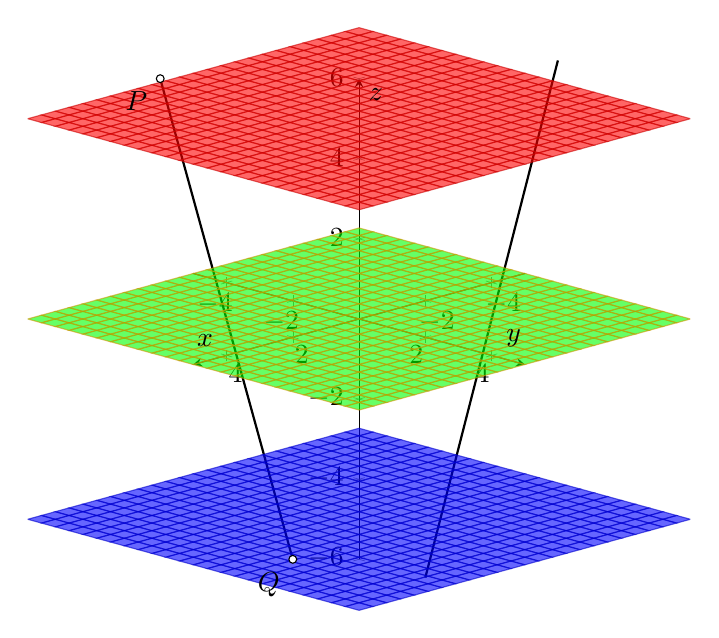
\begin{tikzpicture}
  \begin{axis}[
    width=10cm,
    height=10cm,
    axis lines = middle,
    view={135}{15},
    xlabel={$x$},
    ylabel={$y$},
    zlabel={$z$},
  ]

% Primera la recta
  \addplot3[domain=0:1, samples=2, color=black, thick] ({3 - 2*x}, {-3 + 2*x}, {6 - 12*x});

% Segunda recta
\addplot3[domain=0:1, samples=2, color=black, thick] ({-4 + 4*x}, 2, {6 - 12*x});

% Primer plano
  \addplot3[opacity=0.6, surf, color=blue, domain=-5:5, domain y=-5:5] {-5};

  % Segundo plano
  \addplot3[opacity=0.6, surf, color=green, domain=-5:5, domain y=-5:5] {0};

  % Tercer plano
  \addplot3[opacity=0.6, surf, color=red, domain=-5:5, domain y=-5:5] {5};

  % Puntos de intersección
% Puntos de intersección
% Punto (0,0,0) marcado como P
\node[circle, draw, inner sep=1pt, fill=white] at (axis cs:3,-3,6) [label={-135:$P$}] {};

\node[circle, draw, inner sep=1pt, fill=white] at (axis cs:1,-1,-6) [label={-135:$Q$}] {};



  \end{axis}
\end{tikzpicture}
\end{center}
\end{comment}
    \begin{figure}[H]
        \centering
    \includegraphics[width=0.3\linewidth]{Thales.png}
    \end{figure}

    Entonces, se da el siguiente resultado:
    \begin{equation*}
        \frac{d(s_1,s_2)}{d(s_1,s_3)} =
        \frac{d(r_1,r_2)}{d(r_1,r_3)}
    \end{equation*}
\end{teo}
\begin{proof}
    TERMINAR
\end{proof}


\begin{definicion}
    Sea $E$ un espacio euclídeo. Decimos que $E$ es orientado si $\vec{E}$ tiene definido una orientación.
\end{definicion}


\begin{definicion}
    Sea $E$ un espacio euclídeo orientado. Definimos el ángulo orientado entre los puntos $a,b,c\in E$ como:
    \begin{equation*}
        \theta = \hat{abc} = \measuredangle (\vec{ba},\vec{bc})
    \end{equation*}
    \begin{figure}[H]
        \centering
        \begin{tikzpicture}
          % Dibuja los tres puntos
          \coordinate (B) at (0,0);
          \coordinate (A) at (2,0);
          \coordinate (C) at (1,1.732);
        
          % Dibuja un ángulo theta
          \draw (0.5,0.15) node[above] {$\theta$};
          \draw[-stealth] (0.3,0) arc (0:60:0.3);
        
          % Dibuja líneas que unen los puntos con el vértice theta
          \draw[-stealth] (B) -- (C);
          \draw[-stealth] (B) -- (A);
        
          % Etiqueta los puntos
          \node[below] at (A) {$a$};
          \node[below] at (B) {$b$};
          \node[above] at (C) {$c$};
        \end{tikzpicture}
    \end{figure}

    Hemos de ver que el orden de los puntos es relevante, ya que viene determinado por la orientación.
\end{definicion}

\begin{teo}
    Sea $E$ un espacio euclídeo orientado. Entonces, tenemos que la suma de los tres ángulos de un triángulo es $\pi$:
    \begin{equation*}
        \theta + \gamma + \gamma = \pi
    \end{equation*}
    \begin{figure}[H]
        \centering
        \shorthandoff{"} % Desactivar babel para el carácter " en esta sección
        \begin{tikzpicture}
          % Define las coordenadas de los vértices del triángulo
          \coordinate (A) at (0,0);
          \coordinate (B) at (3,0);
          \coordinate (C) at (1.5,2.598); % Altura de un triángulo equilátero
        
          % Dibuja el triángulo
          \draw (A) -- (B) -- (C) -- cycle;
        
          % Etiqueta los vértices
          \node[below] at (A) {$a$};
          \node[below] at (B) {$b$};
          \node[above] at (C) {$c$};
        
          % Dibuja y etiqueta los ángulos
          \pic["$\alpha$", draw, angle radius=3mm, angle eccentricity=2] {angle = B--A--C};
          \pic["$\beta$", draw, angle radius=3mm, angle eccentricity=2] {angle = C--B--A};
          \pic["$\gamma$", draw, angle radius=3mm, angle eccentricity=2] {angle = A--C--B};
        \end{tikzpicture}
        \shorthandon{"} % Desactivar babel para el carácter " en esta sección
    \end{figure}
\end{teo}
\begin{proof}
    TERMINAR
\end{proof}



\section{Distancia entre subespacios}
\begin{definicion}
    Sea $E$ un espacio euclídeo, y sean $S,T$ dos subespacios euclídeos de $E$. Entonces, se define la distancia entre $S$ y $T$ como:
    \begin{equation*}
        d(S,T) = \inf\{d(p,q)\mid p\in S,~q\in T\}
    \end{equation*}
\end{definicion}

De la definición, se tiene la siguiente proposición de demostración evidente:
\begin{prop}
    Sea $E$ un espacio euclídeo, y sean $S,T$ dos subespacios afines de $E$. Entonces, tenemos que:
    \begin{equation*}
        d(S,T)=0 \Longleftrightarrow S\cap T \neq \emptyset
    \end{equation*}
\end{prop}



\begin{teo}
    Sea $E$ un espacio euclídeo, y sean $S=p+\vec{S}$ y $T=q+\vec{T}$ dos subespacios euclídeos de $E$.

    Se tiene que $\exists p_0\in S,~ q_0\in T$ tal que $\vec{p_0q_0}\in \vec{S}^\perp\cap \vec{T}^\perp = (\vec{S} + \vec{T})^\perp$.

    TERMINAR: VER ESO

    Además, se tiene que $\vec{p_0q_0}$ es único si, y solo si, $\vec{S}\cap \vec{T}=\{0\}$.
\end{teo}
\begin{proof}
    Consideramos $\vec{pq}\in \vec{E}$. Tenemos que $\vec{E}=\vec{S}+\vec{T} \oplus (\vec{S}+\vec{T})^\perp$. Por tanto, tenemos que $\vec{pq}=u+v+w$, con $u\in \vec{S}$, $v\in \vec{T}$, $w\in (\vec{S}+\vec{T})^\perp$. Definimos $q_0=q-v\in T$, $p_0= p+u\in S$, y tenemos que:
    \begin{equation*}
        w = \vec{pq} - u -v = q-p-u-v=q_0-p_0=\vec{p_0q_0} \in (\vec{S} + \vec{T})^\perp = \vec{S}^\perp\cap \vec{T}^\perp
    \end{equation*}

    Respecto a la unicidad, tenemos que $\vec{p_0q_0}$ es único si $u,v$ son únicos. Esto se da si y solo si $\vec{S}\oplus \vec{T}$, y esto se da si y solo si $\vec{S}\cap \vec{T}=\{0\}$.

    TERMINAR
\end{proof}

\begin{coro}\label{coro:dist_ortogonal}
    Sea $E$ un espacio euclídeo, y sean $S=p+\vec{S}$ y $T=q+\vec{T}$ dos subespacios euclídeos de $E$.

    Se tiene que $\exists p_0\in S,~ q_0\in T$ tal que $\vec{p_0q_0}\in \vec{S}^\perp\cap \vec{T}^\perp$ cumpliendo que:
    \begin{equation*}
        d(S,T)=d(p_0,q_0)
    \end{equation*}
\end{coro}
\begin{proof}
    La demostración de la existencia se ha visto en el teorema anterior. Una vez demostrada la existencia, veamos que cumplen la relación de las distancias. Sean $a\in S, b\in T$. Veamos que $d(p_0,q_0)\leq d(a,b)$:
    \begin{multline*}
        d^2(a,b)=\|\vec{ab}\|^2= \langle\vec{ab},\vec{ab}\rangle = 
        \langle\vec{ap_0}+\vec{p_0q_0}+\vec{q_0b},\vec{ap_0}+\vec{p_0q_0}+\vec{q_0b}\rangle = \\=
        \|\vec{ap_0}+\vec{q_0b}\|^2 + \|\vec{p_0q_0}\|^2 + \cancel{2\langle\vec{ap_0}+\vec{q_0b},\vec{p_0q_0}\rangle} \geq \|\vec{p_0q_0}\|^2 = d^2(p_0,q_0)
    \end{multline*}
    donde $\langle\vec{ap_0}+\vec{q_0b},\vec{p_0q_0}\rangle=0$, ya que $\vec{ap_0}\in \vec{S}$ y $\vec{q_0b}\in \vec{T}$.

    Por tanto, tenemos que $d(p_0,q_0)$ es un minorante de $\{d(p,q)\mid p\in S,~q\in T\}$. Además, como $p_0\in S$, $q_0\in T$, tenemos que pertenece al conjunto. Por tanto, no solo es minorante sino que también es el mínimo, por lo que $d(p_0,q_0)$ es el mínimo y, por consecuente, es el ínfimo.
\end{proof}


\begin{ejemplo}
    Sea $\bb{R}^2$ espacio euclídeo, y consideramos
    $$S= (1,1)+\cc{L}\{(1,1)\} \qquad \qquad T= (1,0)+\cc{L}\{(1,1)\}$$ rectas euclídeas. La distancia ambas rectas es:

    TERMINAR
\end{ejemplo}


\begin{ejemplo}
    Sea $\bb{R}^3$ espacio euclídeo, y consideramos $$S= (1,0,1)+\cc{L}\{(1,1, 0)\}\qquad \qquad T= (1,1,0)+\cc{L}\{(-1,1,0)\}$$ rectas euclídeas.

    Usando el corolario \ref{coro:dist_ortogonal}, tenemos que:
    \begin{equation*}
        \vec{pq} = (0,1,-1) = \alpha(1,1,0) + \beta(-1,1,0) + \gamma(0,0,1)
    \end{equation*}
    Resolvemos el sistema para obtener $u,v$.

    Calculamos los puntos $p_0,q_0$ de otra forma. Sean los puntos genéricos de las dos rectas los siguientes:
    \begin{gather*}
        p_\lambda=(1,0,1)+\lambda(1,1,0)=(1+\lambda, \lambda, 1) \in S \\
        q_\mu=(1,1,0)+\mu(-1,1,0)=(1-\mu, 1+\mu, 0) \in T
    \end{gather*}

    Tenemos que $\vec{p_\lambda q_\mu}=(-\mu-\lambda, 1+\mu-\lambda, -1)$. Establecemos que ese vector sea perpendicular a los otros dos:
    \begin{equation*}
        1-2\lambda = 0\Longrightarrow \lambda=\frac{1}{2}
        \qquad
        -1-2\lambda=0 \Longrightarrow \mu = -\frac{1}{2}
    \end{equation*}
\end{ejemplo}



\section{Isometrías}
\begin{definicion}[Isometrías]
    Sea $f:E\to E'$ aplicación afín entre espacios euclídeos. Decimos que $f$ es una isometría o un movimiento rígido si 
    $$d(p,q)=d(f(p),f(q))\qquad \forall p,q\in E$$
\end{definicion}
\begin{ejemplo}
    Sea $E$ en espacio euclídeo, y sea $v\in \vec{E}$. Entonces, $t_v$ es una isometría. Veámoslo:
    \begin{equation*}
        d(t_v(p), t_v(q))=d(p+v, q+v)=\|q-p\|=\|\vec{pq}\|=d(p,q)
    \end{equation*}
\end{ejemplo}

\begin{prop}
    Sean $E,E'$ dos espacios euclídeos, y consideramos $f:E\to E'$. Tenemos que:
    \begin{equation*}
        \langle \vec{f}(v), \vec{f}(w)\rangle = \langle v,w\rangle \Longrightarrow f \text{ es una isometría.}
    \end{equation*}
\end{prop}
Por tanto, tenemos que si $\vec{f}$ es una isometría entre espacios vectoriales, entonces tenemos que $f$ es una isometría.

Recordemos el siguiente lema, tratado en Geometría II:
\begin{lema}
    Sea $\varphi:V^n\to V^{'m}$ aplicación entre espacios vectoriales euclídeos tal que
    $$\langle \varphi(v), \varphi(w)\rangle = \langle v,w\rangle \qquad \forall v,w\in V$$

    Entonces, $\varphi$ es inyectiva y lineal.
\end{lema}


Tenemos por tanto el siguiente teorema:
\begin{teo}
    Sean $E,E'$ dos espacios euclídeos. Consideramos $f:E\to E'$ una isometría. Entonces, tenemos que $f$ es inyectiva, afín y $\vec{f}$ es una isometría vectorial.
\end{teo}


\begin{ejemplo}
    Algunos ejemplos de isometrías son:
    \begin{enumerate}
        \item La identidad
        \item Simetrías $\sigma_S$.

        Tenemos que la matriz asociada a $\vec{\sigma_S}$ en una base ortogonal es diagonal, con $m$ unos y $n$ -1.

        Es decir, su aplicación lineal asociada es la proyección vectorial.
        
        \item Simetrías con desplazamiento $t_v\circ \sigma_S$. Conmuta

        \item Giros $\rho_{O,\theta}$ con centro en $O$ y ángulo $\theta$.
        
        Tenemos que su matriz asociada es un giro. Además, solo tenemos un punto fijo.


        Cómo saber el ángulo de giro sabiendo la matriz $A$. Como la traza es invariante, tenemos que $1+2\cos \theta = tr(A)$.

        \item Movimientos helicoidales $t_v\circ \rho_{O,\rho}$. Conmuta
    \end{enumerate}
\end{ejemplo}

\section{Clasificación de los movimientos}
Sea $f:E^n\to E^n$ un movimiento. Tenemos los siguientes tipos de movimientos:
\begin{itemize}
    \item \ul{Directo}: Conserva la orientación. $|\vec{f}|=1$.
    \item \ul{Inverso}: Invierte la orientación. $|\vec{f}|=-1$.
\end{itemize}

\subsection{Movimientos en el plano $E^2$}

\subsubsection{Movimientos directos}

Tenemos que $\vec{f}$ puede ser $Id$, $-Id$, o un giro de ángulo $\theta\in ]0,\pi[\cup ]\pi,2\pi[$.
\begin{enumerate}
    \item $\vec{f}=Id$: Entonces es una traslación.
    \item $\vec{f}=-Id$: Entonces es una homotecia de razón $-1$.
    \item $\vec{f}=G_{\theta}$: Entonces es un giro.
\end{enumerate}


\subsubsection{Movimientos inversos}

\begin{enumerate}
    \item Simetrías. Recta de puntos fijos.
    \item Simetría con deslizamiento. No hay puntos fijos.
\end{enumerate}

Tenemos por tanto la siguiente tabla:
\begin{table}[H]
    \centering
    \begin{tabular}{c||c|c}
        $P_f\backslash |f|$ & $1$ & $-1$  \\ \hline \hline
        $E^2$ & Identidad & $\times$ \\
        Recta & $\times$ & Reflexión axial \\
        Punto & Giro & $\times$ \\
        $\emptyset$ & Traslación & Reflexión axial con deslizamiento
    \end{tabular}
\end{table}


\subsection{Movimientos en el espacio $E^3$}
\begin{table}[H]
    \centering
    \begin{tabular}{c||c|c}
        $P_f\backslash |f|$ & $1$ & $-1$  \\ \hline \hline
        $E^3$ & Identidad & $\times$ \\
        Plano & $\times$ & Reflexión especular \\
        Recta & Giro & $\times$ \\
        Punto & $\times$ & Reflexión central $\mid$ Giro con simetría \\
        $\emptyset$ & Traslación $\mid$ Helicoidal & Reflexión axial con deslizamiento
    \end{tabular}
\end{table}


\section{Puntos Notables del Triángulo}

Explicar los 4, con dibujos etc.

Importante del baricentro que genera otro triángulo de razón -1/2 o -2.


\begin{teo}[De Euler]
    Demostrado en el pdf. Razón -1/2
\end{teo}